% =====================================================================
%  hookcut - Interaction Walkthrough
%  Compiles with pdfLaTeX on Overleaf. No external assets required.
% =====================================================================
\documentclass[11pt,a4paper]{article}

\usepackage[T1]{fontenc}
\usepackage[utf8]{inputenc}
\usepackage[a4paper,margin=24mm,top=24mm,bottom=26mm]{geometry}
\usepackage{libertine}
\usepackage[scaled=0.82]{beramono}
\usepackage{xcolor}
\usepackage{titlesec}
\usepackage{tcolorbox}
\usepackage{booktabs}
\usepackage{tabularx}
\usepackage{enumitem}
\usepackage{fancyhdr}
\usepackage{microtype}
\usepackage{tikz}
\usepackage[hidelinks]{hyperref}

\usetikzlibrary{positioning,arrows.meta,calc,fit,backgrounds}
\tcbuselibrary{breakable,skins}

% ---------- palette (matches the product) ------------------------------
\definecolor{ink}      {HTML}{16151C}
\definecolor{ink2}     {HTML}{403C4D}
\definecolor{muted}    {HTML}{6D6980}
\definecolor{rulec}    {HTML}{DDD9E7}
\definecolor{cardbg}   {HTML}{F6F4FA}
\definecolor{violet}   {HTML}{5B3FD6}
\definecolor{violetbg} {HTML}{EBE6FB}
\definecolor{magenta}  {HTML}{C42A66}
\definecolor{amber}    {HTML}{9A6212}
\definecolor{teal}     {HTML}{1F7A6C}
\definecolor{cyan}     {HTML}{1D7FA6}

\color{ink}

% ---------- headings ---------------------------------------------------
\titleformat{\section}
  {\sffamily\bfseries\Large\color{ink}}{\thesection}{0.7em}{}
\titleformat{\subsection}
  {\sffamily\bfseries\large\color{ink}}{\thesubsection}{0.6em}{}
\titlespacing*{\section}{0pt}{24pt}{8pt}
\titlespacing*{\subsection}{0pt}{16pt}{5pt}

% ---------- helpers ----------------------------------------------------
\newcommand{\code}[1]{\texttt{\small #1}}
\newcommand{\key}[1]{%
  \tcbox[on line, boxsep=1pt, left=3pt, right=3pt, top=1pt, bottom=1pt,
         colback=cardbg, colframe=rulec, boxrule=0.5pt, arc=2pt]
        {\ttfamily\footnotesize #1}}
\newcommand{\stepnum}[1]{%
  \tikz[baseline=(n.base)]{\node[circle, fill=violet, text=white,
    font=\sffamily\bfseries\footnotesize, inner sep=2pt, minimum size=14pt] (n) {#1};}}

\newtcolorbox{note}[1]{
  enhanced, breakable,
  colback=violetbg, colframe=violetbg,
  boxrule=0pt, arc=3pt,
  left=14pt, right=14pt, top=11pt, bottom=11pt,
  before skip=13pt, after skip=13pt,
  title={\textcolor{violet}{\sffamily\bfseries\scriptsize\MakeUppercase{#1}}},
  attach title to upper={\par\vspace{5pt}}
}

\newtcolorbox{warn}[1]{
  enhanced, breakable,
  colback=cardbg, colframe=magenta,
  boxrule=0pt, leftrule=3pt, arc=0pt, outer arc=0pt,
  left=13pt, right=13pt, top=10pt, bottom=10pt,
  before skip=13pt, after skip=13pt,
  title={\textcolor{magenta}{\sffamily\bfseries\scriptsize\MakeUppercase{#1}}},
  attach title to upper={\par\vspace{5pt}}
}

\setlist[itemize]{leftmargin=1.15em,itemsep=3pt,topsep=4pt}
\setlist[enumerate]{leftmargin=1.5em,itemsep=5pt,topsep=5pt}

% ---------- tikz styles ------------------------------------------------
\tikzset{
  act/.style   = {rounded corners=4pt, fill=violet, text=white,
                  minimum height=12mm, minimum width=25mm, align=center,
                  font=\sffamily\bfseries\scriptsize, inner sep=3pt},
  wait/.style  = {rounded corners=4pt, fill=cardbg, draw=rulec, text=ink2,
                  minimum height=12mm, minimum width=25mm, align=center,
                  font=\sffamily\scriptsize, inner sep=3pt},
  flow/.style  = {-{Stealth[length=2.2mm]}, draw=muted, line width=0.7pt},
  frame/.style = {rounded corners=3pt, draw=rulec, line width=0.7pt},
  fill1/.style = {rounded corners=2pt, fill=cardbg, draw=rulec, line width=0.5pt},
  lbl/.style   = {font=\sffamily\scriptsize, text=ink2, align=center},
  tiny/.style  = {font=\sffamily\tiny, text=muted, align=center},
}

% ---------- running head -----------------------------------------------
\pagestyle{fancy}
\fancyhf{}
\renewcommand{\headrulewidth}{0.4pt}
\fancyhead[L]{\sffamily\scriptsize\color{muted}hookcut --- interaction walkthrough}
\fancyhead[R]{\sffamily\scriptsize\color{muted}\thepage}

\begin{document}

% =====================================================================
\begin{titlepage}
\vspace*{2.4cm}
{\sffamily\bfseries\footnotesize\color{violet}INTERACTION WALKTHROUGH}\par
\vspace{10pt}

{\sffamily\bfseries\fontsize{36}{40}\selectfont
From a finished track\\
\textcolor{muted}{to postable clips}\par}

\vspace{18pt}
{\large\color{ink2}
Every screen, every control, and every keystroke --- in the order an artist
actually meets them.\par}

\vspace{28pt}
\textcolor{rulec}{\rule{\linewidth}{0.6pt}}
\vspace{12pt}

{\ttfamily\small\color{muted}
\begin{tabular}{@{}ll@{}}
Product   & hookcut \\
Repository & Veritron-Innovations/hookcut \\
Branch    & frontend-redesign \\
Scope     & Frontend interaction, upload through download \\
\end{tabular}\par}

\vfill
{\ttfamily\scriptsize\color{muted}
Five steps. Two of them are yours; two are the machine's; one is the hand-off.\par}
\end{titlepage}

\tableofcontents
\newpage

% =====================================================================
\section{The shape of a session}

hookcut is five steps. You act in steps 1, 3 and 5. The machine works in
steps 2 and 4, and you can walk away during both. The whole thing takes about
six minutes for a three-minute song, most of it spent in step 2.

\vspace{14pt}
\begin{center}
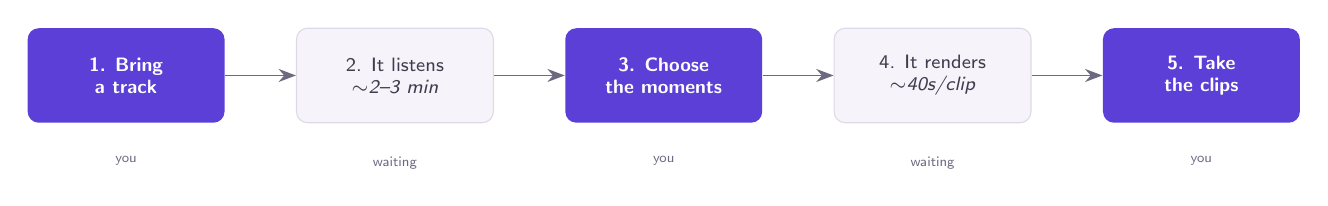
\begin{tikzpicture}[node distance=9mm]
  \node[act]  (s1)                {1. Bring\\a track};
  \node[wait] (s2) [right=of s1]  {2. It listens\\\textit{$\sim$2--3 min}};
  \node[act]  (s3) [right=of s2]  {3. Choose\\the moments};
  \node[wait] (s4) [right=of s3]  {4. It renders\\\textit{$\sim$40s/clip}};
  \node[act]  (s5) [right=of s4]  {5. Take\\the clips};

  \draw[flow] (s1) -- (s2);
  \draw[flow] (s2) -- (s3);
  \draw[flow] (s3) -- (s4);
  \draw[flow] (s4) -- (s5);

  \node[tiny, below=3mm of s1] {you};
  \node[tiny, below=3mm of s2] {waiting};
  \node[tiny, below=3mm of s3] {you};
  \node[tiny, below=3mm of s4] {waiting};
  \node[tiny, below=3mm of s5] {you};
\end{tikzpicture}
\end{center}

\vspace{10pt}
A rail across the top of the app shows which step you are on at all times,
labelled \textbf{Listen \textperiodcentered{} Find \textperiodcentered{}
Choose \textperiodcentered{} Render \textperiodcentered{} Done}. A gradient
pill slides along it, and pulses while something is running.

\begin{note}{The one thing to understand}
Nothing is rendered until you say so. Step 2 only transcribes and analyses ---
both comparatively quick and cheap. The expensive part, step 4, runs on the
moments you approved and nothing else. If the machine picks badly, you find
out before any time is spent on it, not after.
\end{note}

% =====================================================================
\section{Step 1 --- Bring a track}

\subsection{What you see}

\begin{center}
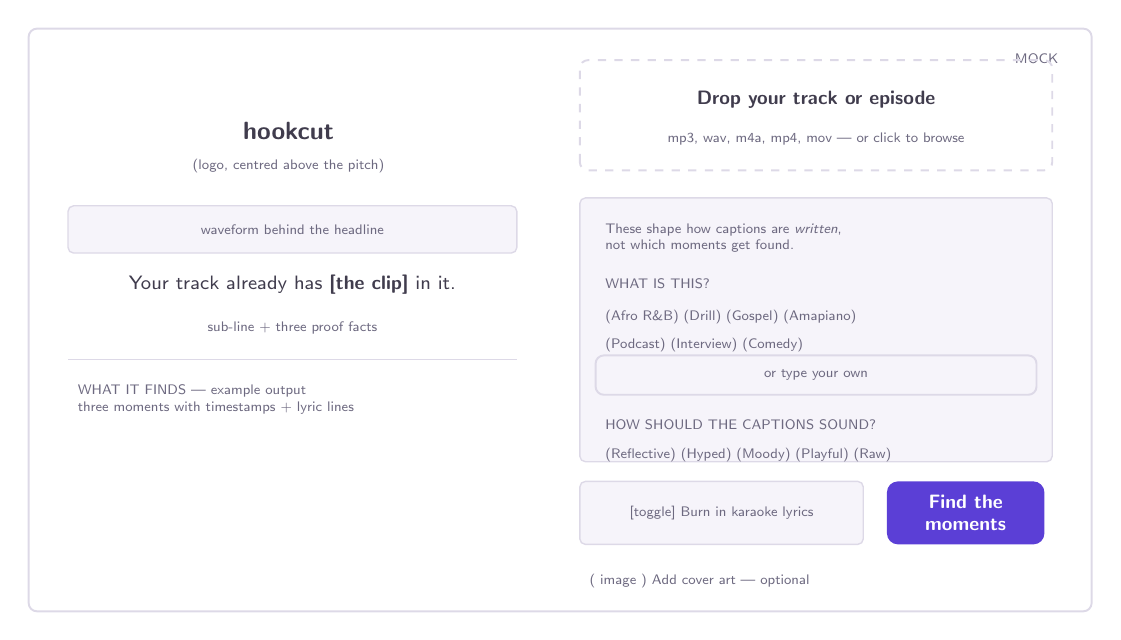
\begin{tikzpicture}[scale=1]
  % outer frame
  \draw[frame] (0,0) rectangle (13.5,7.4);
  % masthead
  \node[tiny, anchor=north east] at (13.2,7.2) {MOCK};

  % left column
  \node[lbl, font=\sffamily\bfseries\small] at (3.3,6.1) {hookcut};
  \node[tiny] at (3.3,5.65) {(logo, centred above the pitch)};
  \draw[fill1] (0.5,4.55) rectangle (6.2,5.15);
  \node[tiny] at (3.35,4.85) {waveform behind the headline};
  \node[lbl] at (3.35,4.15) {Your track already has \textbf{[the clip]} in it.};
  \node[tiny] at (3.35,3.6) {sub-line + three proof facts};
  \draw[rulec] (0.5,3.2) -- (6.2,3.2);
  \node[tiny, align=left, anchor=north west] at (0.5,3.0)
    {WHAT IT FINDS \textemdash{} example output\\
     three moments with timestamps + lyric lines};

  % right column
  \draw[frame, dashed] (7.0,5.6) rectangle (13.0,7.0);
  \node[lbl] at (10.0,6.5) {\textbf{Drop your track or episode}};
  \node[tiny] at (10.0,6.0) {mp3, wav, m4a, mp4, mov --- or click to browse};

  \draw[fill1] (7.0,1.9) rectangle (13.0,5.25);
  \node[tiny, anchor=north west, align=left] at (7.2,5.05)
    {These shape how captions are \textit{written},\\not which moments get found.};
  \node[tiny, anchor=north west] at (7.2,4.35) {WHAT IS THIS?};
  \node[tiny, anchor=north west] at (7.2,3.95)
    {(Afro R\&B) (Drill) (Gospel) (Amapiano)};
  \node[tiny, anchor=north west] at (7.2,3.6) {(Podcast) (Interview) (Comedy)};
  \draw[frame] (7.2,2.75) rectangle (12.8,3.25);
  \node[tiny] at (10.0,3.0) {or type your own};
  \node[tiny, anchor=north west] at (7.2,2.55) {HOW SHOULD THE CAPTIONS SOUND?};
  \node[tiny, anchor=north west] at (7.2,2.2)
    {(Reflective) (Hyped) (Moody) (Playful) (Raw)};

  \draw[fill1] (7.0,0.85) rectangle (10.6,1.65);
  \node[tiny] at (8.8,1.25) {[toggle] Burn in karaoke lyrics};
  \node[act, minimum width=20mm, minimum height=8mm] at (11.9,1.25) {Find the\\moments};

  \node[tiny, anchor=north west] at (7.0,0.6) {( image ) Add cover art \textemdash{} optional};
\end{tikzpicture}
\end{center}

\subsection{What each control actually does}

\begin{tabularx}{\linewidth}{@{}p{3.4cm} X@{}}
\toprule
{\sffamily\footnotesize\color{muted}CONTROL} &
{\sffamily\footnotesize\color{muted}EFFECT} \\
\midrule
Drop zone &
\small Accepts a drag-and-drop or a click. Audio (\code{mp3 wav m4a flac aac ogg})
takes the song path; anything else takes the video path. Once a file lands it
shows the name and size, and you can drop another to swap it. \\[4pt]

What is this? &
\small Tells the model whether to hunt for a chorus or for spoken beats, and
sets the register the captions are written in. Tap a chip, or type your own.
Tap an active chip again to clear it. \\[4pt]

How should the captions sound? &
\small Sets tone only. Neither this nor the genre changes \textit{which}
moments get found --- that is what step 3 is for. \\[4pt]

Burn in karaoke lyrics &
\small Song sources only. A video source keeps its own picture, so the switch
has no effect there. \\[4pt]

Add cover art &
\small Optional. Without it, hookcut falls back to the artwork embedded in the
mp3's ID3 tags; failing that, a plain background. \\[4pt]

Find the moments &
\small Uploads and starts step 2. Disabled until a file is chosen. \\
\bottomrule
\end{tabularx}

\begin{note}{You are not asked how many clips you want}
Earlier versions asked for a number up front. They no longer do: hookcut looks
for a generous spread and you narrow it in step 3, where you can hear each one
first. Choosing blind was the worse version of a decision you are about to make
properly.
\end{note}

% =====================================================================
\section{Step 2 --- While it listens}

Nothing is required of you here. You can switch tabs; the job runs on the
server.

\vspace{10pt}
\begin{center}
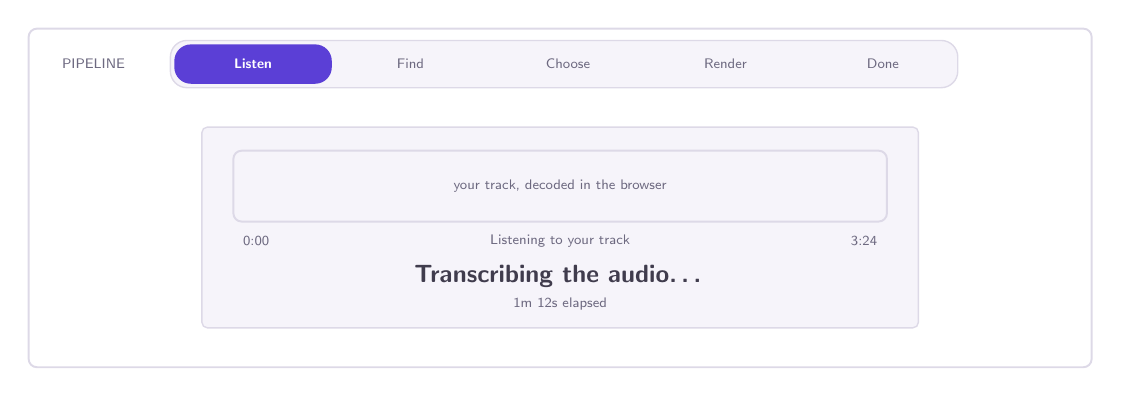
\begin{tikzpicture}
  \draw[frame] (0,0) rectangle (13.5,4.3);

  % rail
  \node[tiny, anchor=west] at (0.3,3.85) {PIPELINE};
  \draw[fill1, rounded corners=6pt] (1.8,3.55) rectangle (11.8,4.15);
  \draw[rounded corners=6pt, fill=violet, draw=none] (1.85,3.6) rectangle (3.85,4.1);
  \node[font=\sffamily\bfseries\tiny, text=white] at (2.85,3.85) {Listen};
  \node[tiny] at (4.85,3.85) {Find};
  \node[tiny] at (6.85,3.85) {Choose};
  \node[tiny] at (8.85,3.85) {Render};
  \node[tiny] at (10.85,3.85) {Done};

  % panel
  \draw[fill1] (2.2,0.5) rectangle (11.3,3.05);
  \draw[frame] (2.6,1.85) rectangle (10.9,2.75);
  \node[tiny] at (6.75,2.3) {your track, decoded in the browser};
  \node[tiny, anchor=west] at (2.6,1.6) {0:00};
  \node[tiny] at (6.75,1.6) {Listening to your track};
  \node[tiny, anchor=east] at (10.9,1.6) {3:24};
  \node[lbl, font=\sffamily\bfseries\small] at (6.75,1.15) {Transcribing the audio\ldots};
  \node[tiny] at (6.75,0.8) {1m 12s elapsed};
\end{tikzpicture}
\end{center}

\begin{itemize}
\item The waveform is \textbf{your} file, decoded locally in the browser --- no
      upload round trip, real peaks, real duration.
\item The stage label and elapsed counter are the honest signals: hookcut does
      not report a percentage because Whisper does not produce one.
\item Transcription is the long part. A three-minute song is roughly one to
      three minutes on a laptop CPU.
\end{itemize}

\begin{warn}{Not yet live}
Found moments are wired to light up on this waveform as they arrive, but the
backend currently returns all concepts in one batch at the end. Until it
streams partial results, the waveform stays empty during the wait and every
moment appears at once when step 3 opens.
\end{warn}

% =====================================================================
\section{Step 3 --- Choose the moments}

This is the screen that matters. Everything on it is real: your audio, your
transcript, your cover art.

\vspace{10pt}
\begin{center}
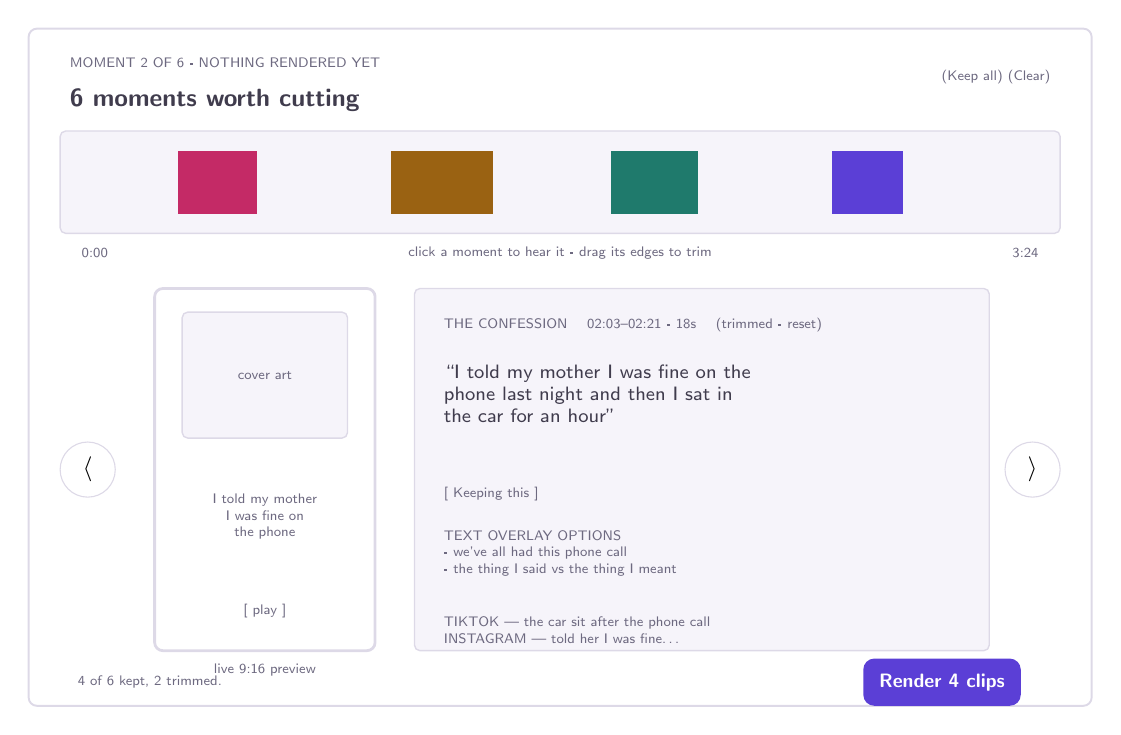
\begin{tikzpicture}
  \draw[frame] (0,0) rectangle (13.5,8.6);

  % header
  \node[tiny, anchor=north west] at (0.4,8.35) {MOMENT 2 OF 6 \textperiodcentered{} NOTHING RENDERED YET};
  \node[lbl, anchor=north west, font=\sffamily\bfseries\small] at (0.4,7.95)
    {6 moments worth cutting};
  \node[tiny, anchor=north east] at (13.1,8.2) {(Keep all) (Clear)};

  % waveform with regions
  \draw[fill1] (0.4,6.0) rectangle (13.1,7.3);
  \draw[fill=magenta, draw=none] (1.9,6.25) rectangle (2.9,7.05);
  \draw[fill=amber,   draw=none] (4.6,6.25) rectangle (5.9,7.05);
  \draw[fill=teal,    draw=none] (7.4,6.25) rectangle (8.5,7.05);
  \draw[fill=violet,  draw=none] (10.2,6.25) rectangle (11.1,7.05);
  \node[tiny, anchor=west] at (0.55,5.75) {0:00};
  \node[tiny] at (6.75,5.75) {click a moment to hear it \textperiodcentered{} drag its edges to trim};
  \node[tiny, anchor=east] at (12.95,5.75) {3:24};

  % arrows
  \node[circle, draw=rulec, minimum size=7mm, font=\small] at (0.75,3.0) {$\langle$};
  \node[circle, draw=rulec, minimum size=7mm, font=\small] at (12.75,3.0) {$\rangle$};

  % preview frame (9:16)
  \draw[frame, line width=1pt] (1.6,0.7) rectangle (4.4,5.3);
  \draw[fill1] (1.95,3.4) rectangle (4.05,5.0);
  \node[tiny] at (3.0,4.2) {cover art};
  \node[tiny, align=center] at (3.0,2.4) {I told my mother\\I was fine on\\the phone};
  \node[tiny] at (3.0,1.2) {[ play ]};
  \node[tiny] at (3.0,0.45) {live 9:16 preview};

  % detail card
  \draw[fill1] (4.9,0.7) rectangle (12.2,5.3);
  \node[tiny, anchor=north west] at (5.15,5.05) {THE CONFESSION \quad 02:03--02:21 \textperiodcentered{} 18s \quad (trimmed \textperiodcentered{} reset)};
  \node[lbl, anchor=north west, align=left] at (5.15,4.45)
    {``I told my mother I was fine on the\\phone last night and then I sat in\\the car for an hour''};
  \node[tiny, anchor=north west] at (5.15,2.9) {[ Keeping this ]};
  \node[tiny, anchor=north west, align=left] at (5.15,2.35)
    {TEXT OVERLAY OPTIONS\\
     \textperiodcentered{} we've all had this phone call\\
     \textperiodcentered{} the thing I said vs the thing I meant};
  \node[tiny, anchor=north west, align=left] at (5.15,1.25)
    {TIKTOK \textemdash{} the car sit after the phone call\\
     INSTAGRAM \textemdash{} told her I was fine\ldots};

  % dock
  \node[tiny, anchor=west] at (0.5,0.3) {4 of 6 kept, 2 trimmed.};
  \node[act, minimum width=20mm, minimum height=6mm] at (11.6,0.3) {Render 4 clips};
\end{tikzpicture}
\end{center}

\subsection{The three things you can do}

\begin{enumerate}
\item \textbf{Hear it.} Click a coloured region on the waveform, or press play
      on the preview. It plays that exact range and stops at the out-point. A
      white playhead sweeps the waveform while it runs.

\item \textbf{Trim it.} The active moment has a grab handle at each edge. Drag
      an edge to move the in or out point; drag the middle to slide the whole
      window without changing its length. The timestamp updates live and a
      \textbf{trimmed \textperiodcentered{} reset} chip appears --- click it to
      go back to the model's original pick. Clips are held between 5 and 60
      seconds.

\item \textbf{Keep or skip it.} Everything starts kept. Press \emph{Skip this
      one} to drop a moment; its region dims on the waveform so your whole set
      of decisions reads at a glance.
\end{enumerate}

\subsection{The preview is the clip}

The 9:16 frame is a browser rebuild of what the renderer will composite: the
blurred cover-art bleed, the sharp art above centre, and the lyric burning in
word by word. Press play and the words light up in time with your audio.

\begin{note}{What the preview gets exactly right, and what it approximates}
The art, the framing, the audio and the cut points are exact. The word-by-word
timing is estimated in the browser --- words are spread across the range by
length. The rendered clip uses Whisper's real per-word timestamps, so the final
sync is tighter than the preview shows. The caption under the frame says so.
\end{note}

\subsection{Moving through the deck}

One moment fills the screen at a time. Move with the \key{$\leftarrow$} and
\key{$\rightarrow$} arrow keys, the chevrons either side, or by clicking any
region on the waveform. The waveform is the overview --- all moments, in the
positions they occupy in the song --- so nothing is hidden by showing one at a
time.

When you are happy, press \textbf{Render N clips}. Only the kept moments, at
whatever cut points you set, are sent.

% =====================================================================
\section{Step 4 --- While it renders}

The same screen furniture as step 2, with the rail now on \textbf{Render}.
Roughly forty seconds per clip for a song, because each one is a full video
encode. Video sources are far faster --- they are stream-copied, not
re-encoded.

% =====================================================================
\section{Step 5 --- Take the clips}

\begin{center}
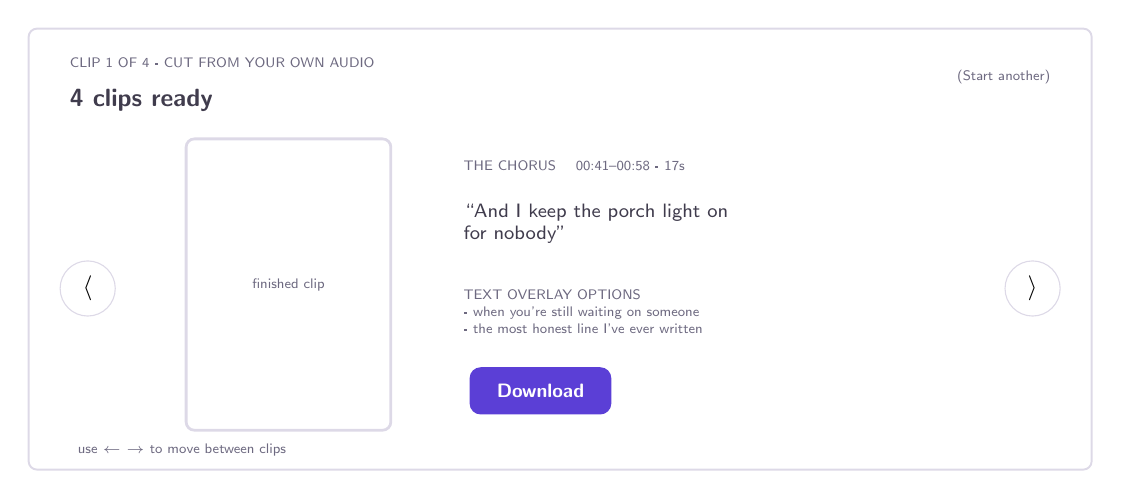
\begin{tikzpicture}
  \draw[frame] (0,0) rectangle (13.5,5.6);
  \node[tiny, anchor=north west] at (0.4,5.35) {CLIP 1 OF 4 \textperiodcentered{} CUT FROM YOUR OWN AUDIO};
  \node[lbl, anchor=north west, font=\sffamily\bfseries\small] at (0.4,4.95) {4 clips ready};
  \node[tiny, anchor=north east] at (13.1,5.2) {(Start another)};

  \node[circle, draw=rulec, minimum size=7mm, font=\small] at (0.75,2.3) {$\langle$};
  \node[circle, draw=rulec, minimum size=7mm, font=\small] at (12.75,2.3) {$\rangle$};

  \draw[frame, line width=1pt] (2.0,0.5) rectangle (4.6,4.2);
  \node[tiny] at (3.3,2.35) {finished clip};

  \node[tiny, anchor=north west] at (5.4,4.05) {THE CHORUS \quad 00:41--00:58 \textperiodcentered{} 17s};
  \node[lbl, anchor=north west, align=left] at (5.4,3.5)
    {``And I keep the porch light on\\for nobody''};
  \node[tiny, anchor=north west, align=left] at (5.4,2.4)
    {TEXT OVERLAY OPTIONS\\
     \textperiodcentered{} when you're still waiting on someone\\
     \textperiodcentered{} the most honest line I've ever written};
  \node[act, minimum width=18mm, minimum height=6mm] at (6.5,1.0) {Download};

  \node[tiny, anchor=west] at (0.5,0.25) {use $\leftarrow$ $\rightarrow$ to move between clips};
\end{tikzpicture}
\end{center}

One clip at a time, at its true aspect ratio --- 9:16 for songs, the source
ratio for video. Play it in place, read its captions and overlay options, and
download it. \textbf{Start another} clears everything and returns to step 1.

\begin{warn}{Where the flow still ends early}
The overlay hooks are written but not burned into the video, so putting text on
screen still means opening an editor. Captions have no copy button, and there is
no batch download. Those three gaps are the difference between hookcut producing
\textit{clips} and hookcut producing \textit{posts}.
\end{warn}

% =====================================================================
\section{Keyboard and pointer reference}

\begin{tabularx}{\linewidth}{@{}p{3.6cm} p{3.4cm} X@{}}
\toprule
{\sffamily\footnotesize\color{muted}INPUT} &
{\sffamily\footnotesize\color{muted}WHERE} &
{\sffamily\footnotesize\color{muted}DOES} \\
\midrule
\key{$\leftarrow$} \key{$\rightarrow$} & Steps 3 and 5 & \small Previous / next moment or clip. Ignored while typing in a field. \\[3pt]
\key{$\leftarrow$} \key{$\rightarrow$} & Focused trim handle & \small Nudges that edge by 0.25\,s. \\[3pt]
\key{Shift} + arrows & Focused trim handle & \small Nudges by 1\,s. \\[3pt]
\key{Tab} & Everywhere & \small Moves through controls; focus is always visible. \\[3pt]
Click a region & Step 3 waveform & \small Selects that moment and plays its exact range. \\[3pt]
Drag an edge & Step 3 waveform & \small Trims the in or out point. \\[3pt]
Drag the middle & Step 3 waveform & \small Slides the window, keeping its length. \\[3pt]
Click the preview & Step 3 & \small Play / pause. \\[3pt]
Drag a file & Step 1 & \small Drops it straight onto the target. \\
\bottomrule
\end{tabularx}

% =====================================================================
\section{When something goes wrong}

Every failure resolves to a message and a way out --- there is no state that
spins forever.

\begin{tabularx}{\linewidth}{@{}p{5.0cm} X@{}}
\toprule
{\sffamily\footnotesize\color{muted}SITUATION} &
{\sffamily\footnotesize\color{muted}WHAT YOU SEE} \\
\midrule
Backend not running &
\small ``Couldn't reach the backend'', with the command to start it, and a
\emph{Start over} button. \\[4pt]
Backend restarts mid-job &
\small The job is gone from memory, so you get ``Job not found. The server may
have restarted'', not a spinner. \\[4pt]
Connection drops while polling &
\small ``Lost contact with the backend'' --- polling stops rather than
retrying silently. \\[4pt]
ffmpeg or the model fails &
\small The server's own error text, verbatim, on the error screen. \\[4pt]
Nothing kept in step 3 &
\small The render button disables and the dock reads ``Nothing kept yet.'' \\
\bottomrule
\end{tabularx}

\begin{warn}{One real limitation}
A running job lives only in the browser tab that started it. Refreshing, or
closing the tab, loses access to it --- the job id is held in memory and is not
in the URL. The work continues on the server, but the interface cannot find its
way back.
\end{warn}

% =====================================================================
\section{Running it without a backend}

The frontend ships with a mock layer so the whole interface can be driven with
no Python and no ffmpeg.

\begin{enumerate}
\item Create \code{frontend/.env.local} containing \code{NEXT\_PUBLIC\_MOCK=1}
\item \code{npm run dev} --- the port is pinned to 3002
\item A \textbf{mock} chip appears top right; press \key{`} to open it
\end{enumerate}

Jump straight to any screen with \code{?state=working}, \code{?state=review},
\code{?state=rendering}, \code{?state=done} or \code{?state=error}. The mock
walks the full stage sequence in about eleven seconds.

\begin{note}{What is real in mock mode}
The layout, the interactions, the trim handles and the deck all behave exactly
as they do for real. The waveform is synthetic and playback is disabled, because
there is no file behind a seeded job. Drop an actual mp3 on step 1 and the
waveform, the audio and the live preview all become real --- the backend is only
needed from the moment you press \emph{Find the moments}.
\end{note}

\end{document}
